\begin{frame}{周期外力のあるRösslerモデル}
    \vspace{-.35cm}
    % スライドを2つの列に分割
    \begin{columns}[T] % [T] は列を上部で揃えるオプション
  
      \begin{column}{.5\textwidth}
        \begin{block}{Rössler方程式}
            次の方程式を解くことで時系列データを生成する.
            \begin{align}
                \frac{dx}{dt} &= -y - z + P(t)\\
                \frac{dy}{dt} &= x + ay \\
                \frac{dz}{dt} &= b + z(x - c)
            \end{align}
            ここで,$P(t) := A \sin(t + \theta_p(t))$ とする.
           
            ただし,$p \in \left\{ n \in \Z \mid -12 \leq n \leq 12 \right\}$ とし,
            $\theta_p$ は $4$ 日に $1$ 度外力の位相を $p\cdot 2\pi/24$ だけ早めるような関数.
        \end{block}
      \end{column}
      \begin{column}{.5\textwidth}
        \vspace{-.6cm}
        \begin{figure}
            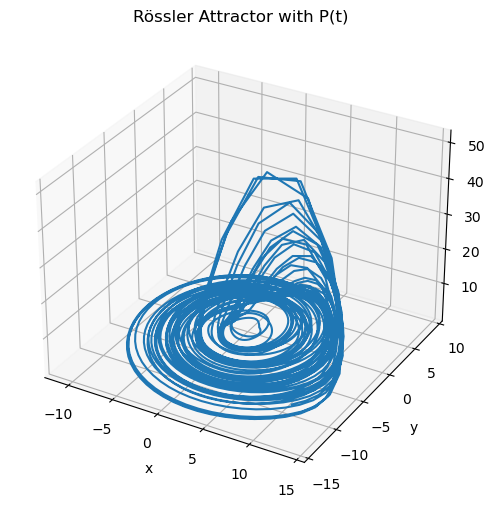
\includegraphics[width=0.9\textwidth]{Fig/NEWrossler_attractor.png}
            \caption{\scriptsize{Rösslerモデル}}
        \end{figure}
        
      \end{column}
    \end{columns}
  \end{frame}


  \begin{frame}{Reservoir Computer を用いたカオス予測手法}
    % スライドを2つの列に分割
    \begin{columns}[T] % [T] は列を上部で揃えるオプション
    
        \begin{column}{.5\textwidth}
        \vspace{-.35cm}
        % ここに右側のコンテンツを配置
        \begin{block}{予測の手法}
          \begin{enumerate}
            \item 予測する系の時系列データを生成\begin{itemize}
              \item 外力付きのRössler方程式の系の場合,変数 $X_t, Y_t$ と外力 $P_t$ から成る配列.
            \end{itemize}
            \item ReserviorのHyperparameterの最適化\begin{itemize}
              \item train 期間 で学習を行い,test期間で
              
              教師付きの予測を行う.
              \item test 期間での予測値と真の値との誤差を目的関数として,最適化を行う.
            \end{itemize}
            \item self-evolve 予測を行う.\begin{itemize}
              \item train, warm-up 期間 の後,
              Reservoir に未来予測をさせる.
              \item 各ステップの入力は,Reserviorの一期前の出力に対して,外力の真の値だけ
              
              修正した配列.
            \end{itemize}
        \end{enumerate}
        \end{block}
        \end{column}
    
        \begin{column}{.5\textwidth}
        \begin{figure}
            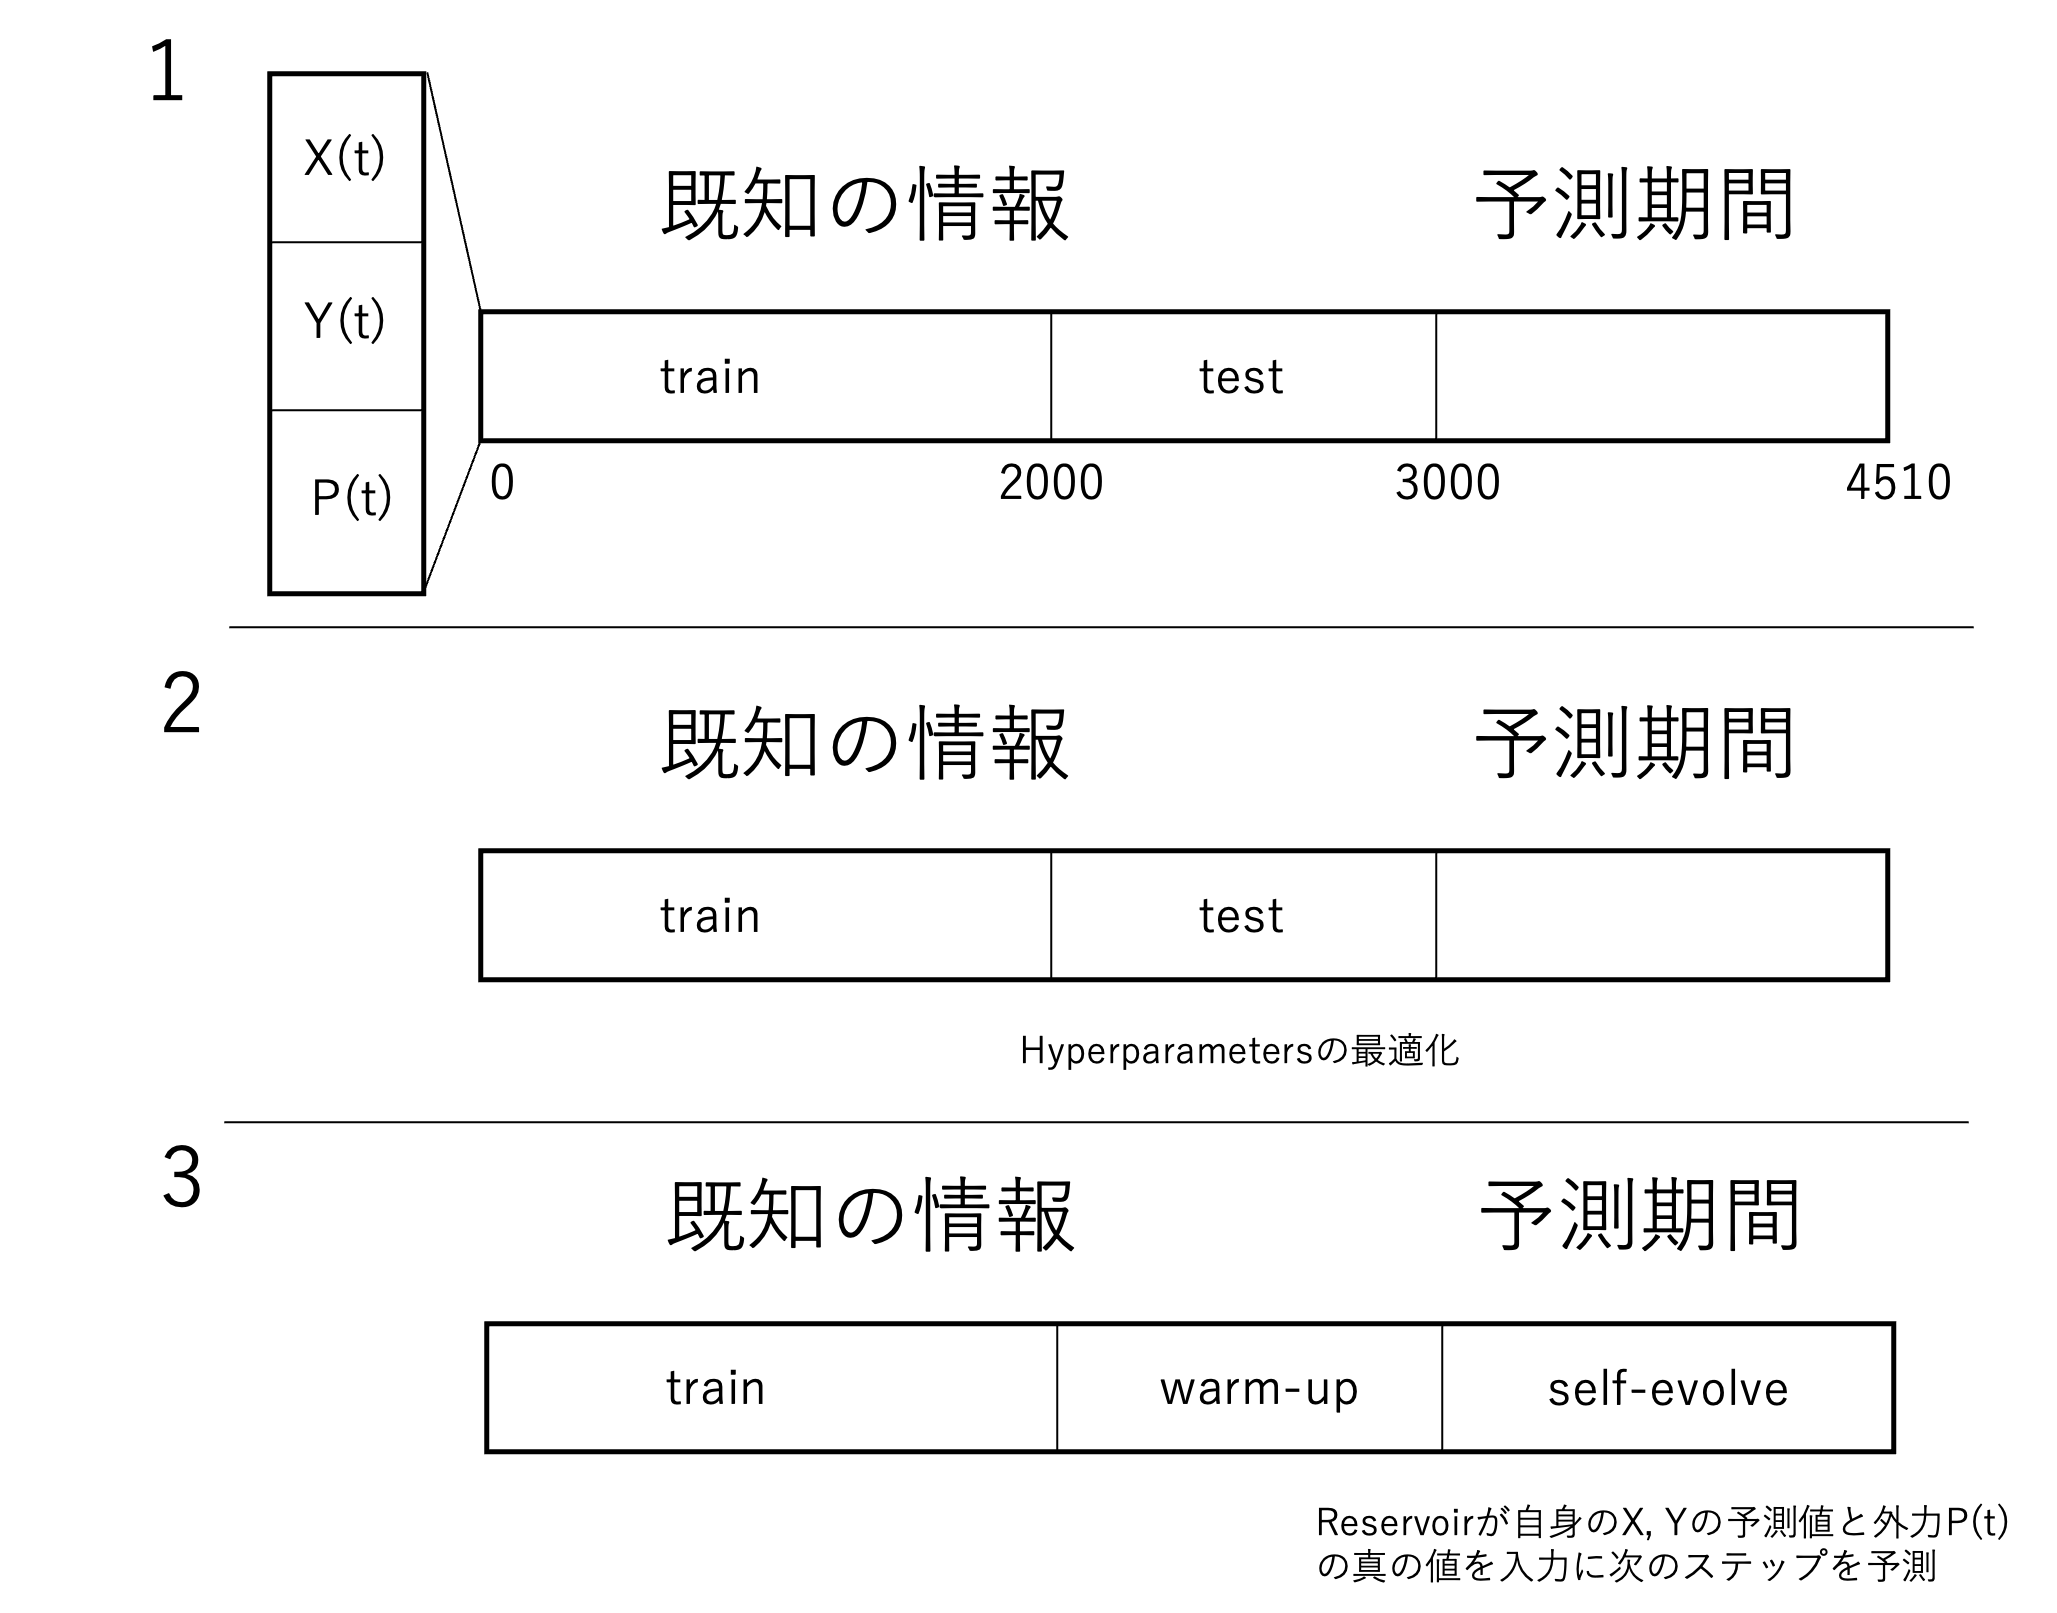
\includegraphics[width=\textwidth]{Fig/please.png}
            \caption{\scriptsize{Reservoir Computer を用いたカオス予測の手順}}
        \end{figure}   
        \end{column}
    \end{columns}
    \end{frame}

\begin{frame}{未知の外力に対する Resever Computer の性能}
    \begin{columns}[T] % [T] は列を上部で揃えるオプション
        \begin{column}{.5\textwidth}
            \begin{itemize}
                \item Hyperparameter の最適化は位相シフトが$8$時間である系に対して行う.
                \item その後,同じ Reservoir で異なる位相シフトを持つ系に対しても予測を行う.\begin{itemize}
                    \item 未知の外力に対するReservoir の予測性能を測る.
                \end{itemize}
            \end{itemize}
            
            \vspace{-.5em}
            \begin{figure}
                %\centering % 画像を中央揃えにする(オプション)
                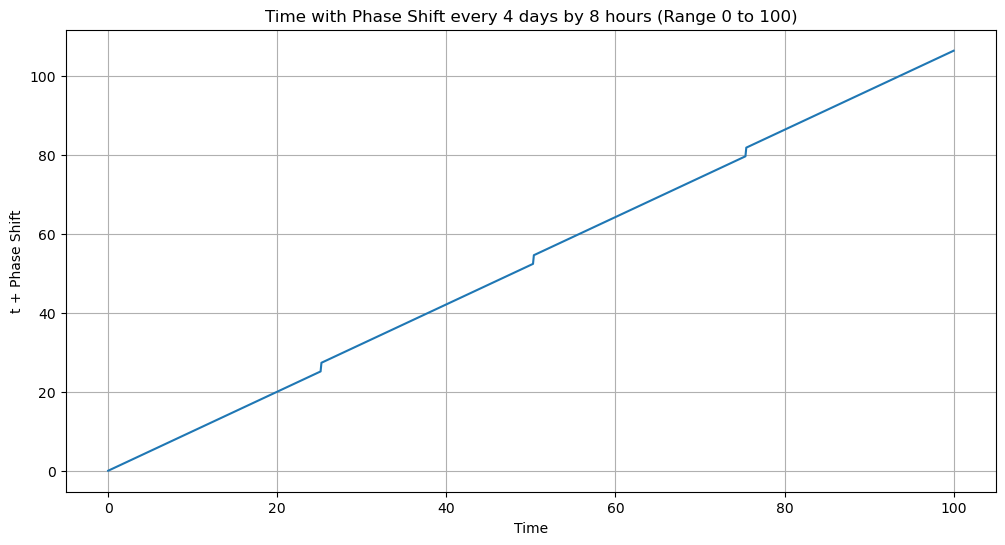
\includegraphics[width=0.8\textwidth]{Fig/phase_shift_plot.png}
                \caption{\scriptsize{$4$ 日に一度 $8$ 時間早めたときの外力の位相}}
            \end{figure}
        \end{column}
        \begin{column}{.5\textwidth}
            \begin{figure}
                %\centering % 画像を中央揃えにする(オプション)
                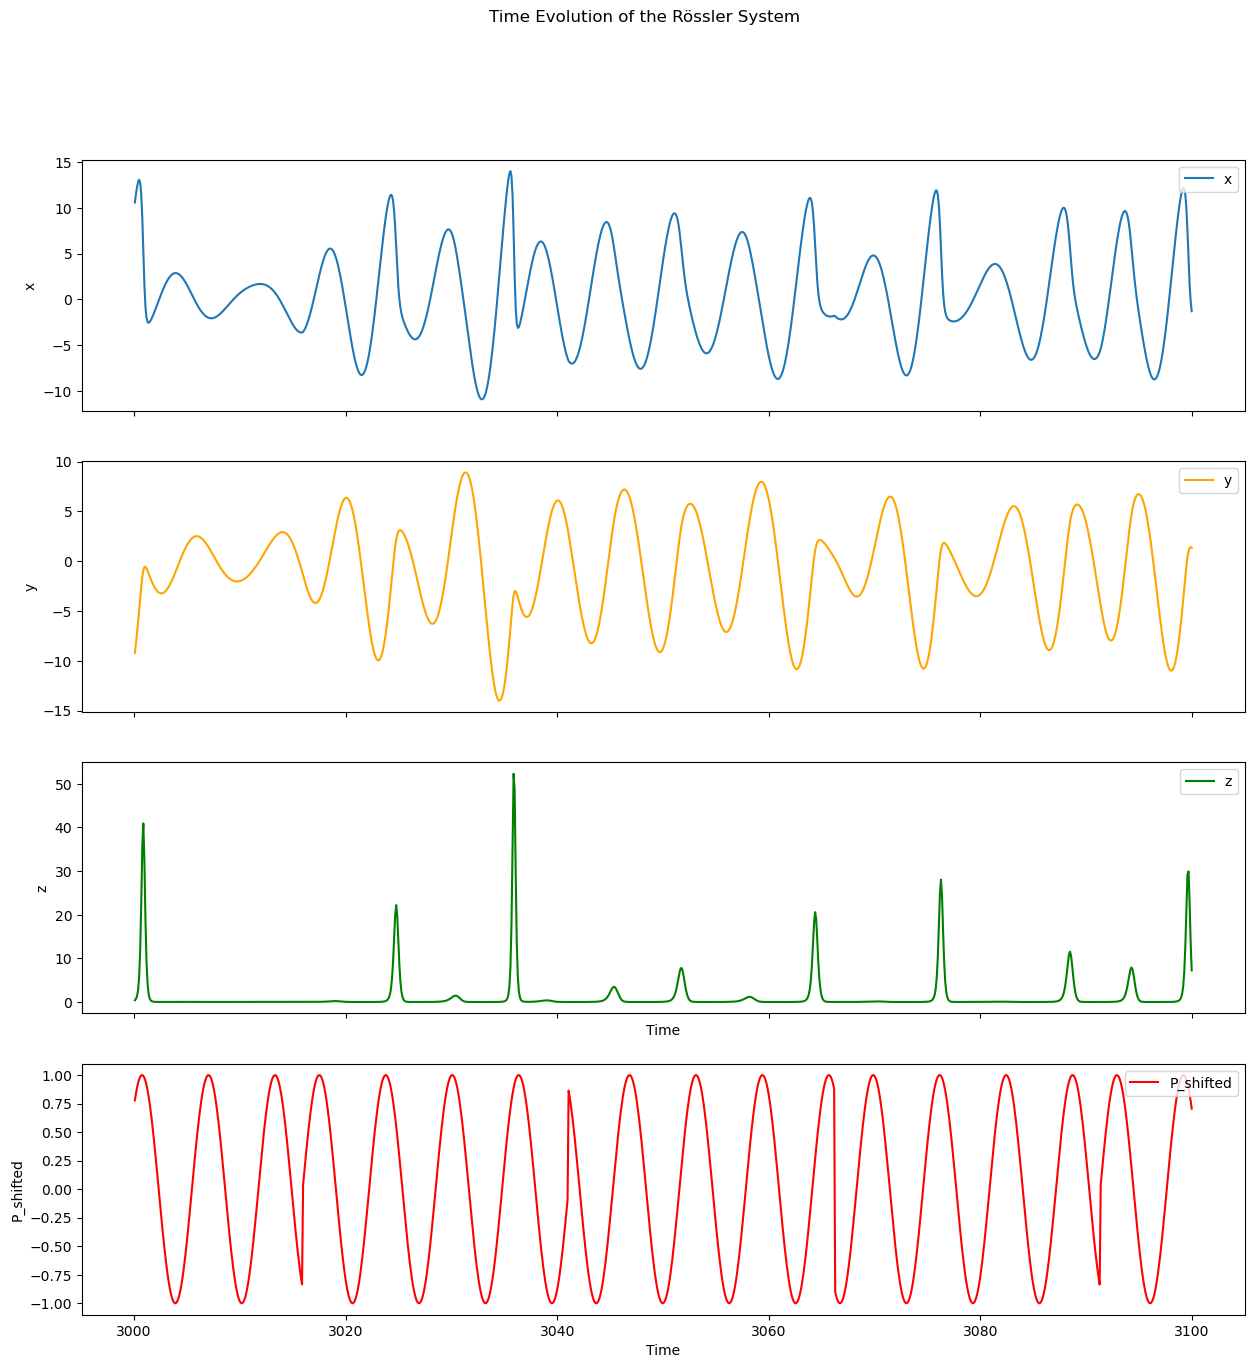
\includegraphics[width=0.7\textwidth]{Fig/NEWrossler_waves.png}
                \caption{\scriptsize{位相シフト(8時間分)のある周期外力付きのRössler システム:上から $x, y, z, P(t)$. }}
            \end{figure}
        \end{column}
      \end{columns}
    
\end{frame}


\section{結果}
\begin{frame}{予測結果}
  \begin{columns}[T] % [T] は列を上部で揃えるオプション
    \begin{column}{.5\textwidth}
      \begin{figure}
        \vspace{-.5cm}
        % 画像1
        \begin{minipage}[c][.27\textheight][c]{\linewidth}
          \centering
          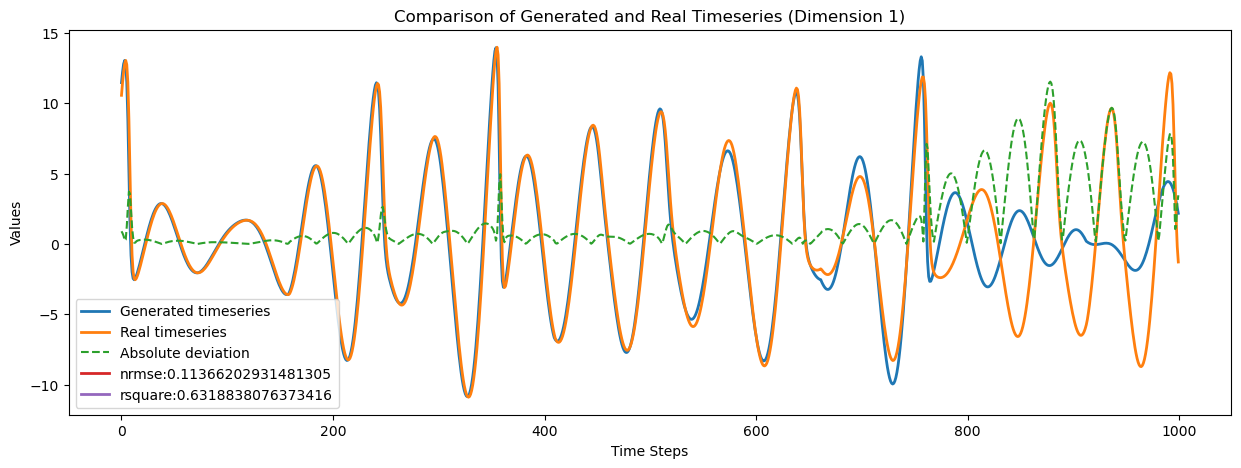
\includegraphics[width=0.7\linewidth]{Fig/8.x.png}
        \end{minipage}
    
        \vspace{-.5em}

        % 画像2
        \begin{minipage}[c][.27\textheight][c]{\linewidth}
          \centering
          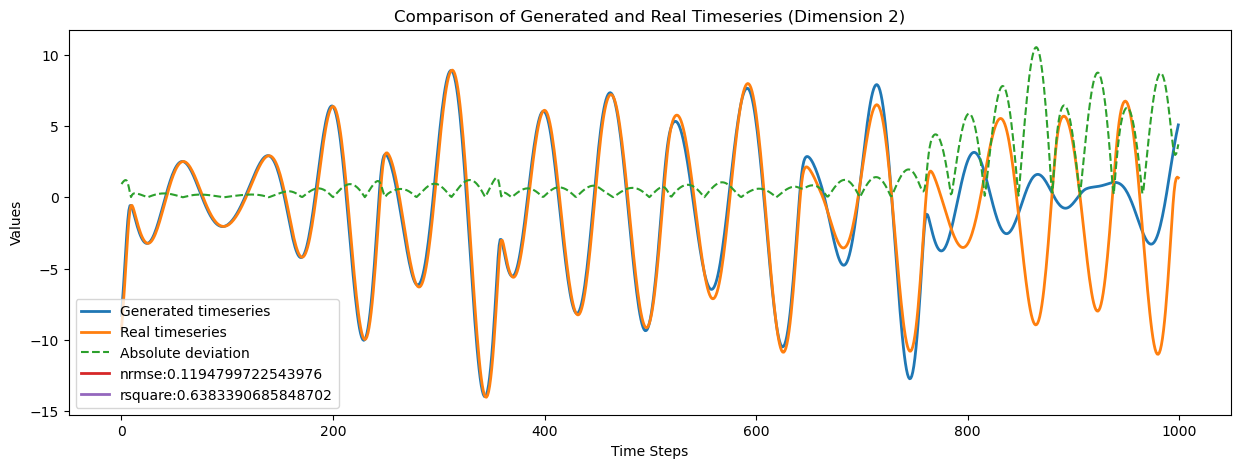
\includegraphics[width=0.7\linewidth]{Fig/8.y.png}
        \end{minipage}
        
        \vspace{.5em}
        % 画像3
        \begin{minipage}[c][.27\textheight][c]{\linewidth}
          \centering
          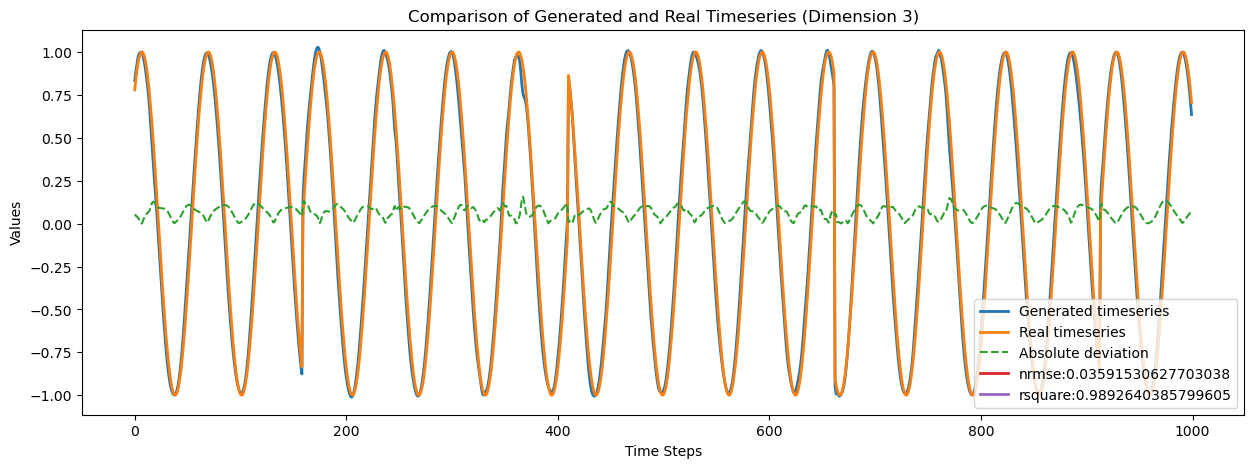
\includegraphics[width=0.7\linewidth]{Fig/8.p.png}
          \caption{\scriptsize{位相シフト(8時間分)のある外力付きRösslerモデルの予測.上から $x, y, P(t)$. }}
        \end{minipage}
      \end{figure}
    \end{column}
    \begin{column}{.5\textwidth}
      \begin{figure}
        \vspace{-.5cm}
        % 画像1
        \begin{minipage}[c][.27\textheight][c]{\linewidth}
          \centering
          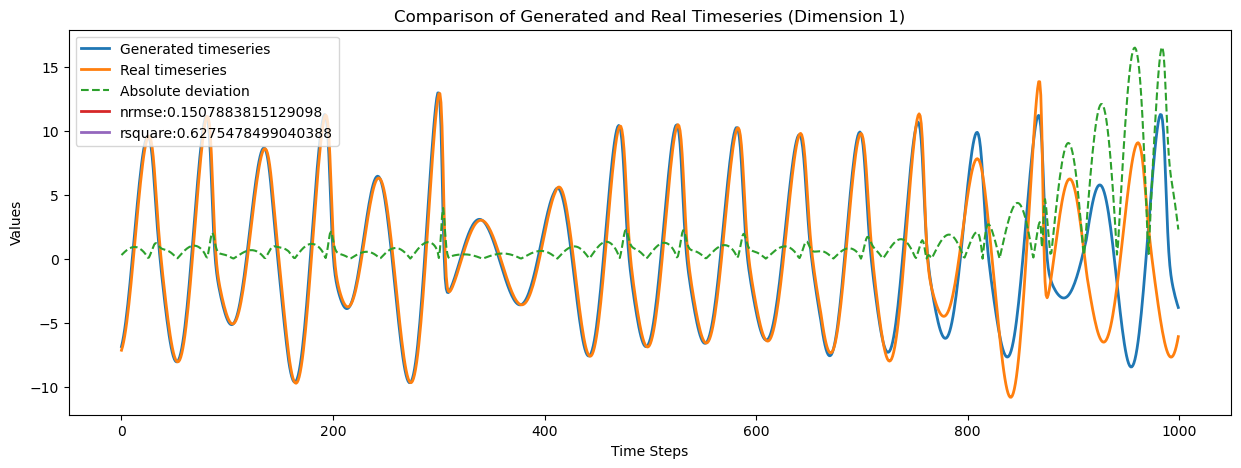
\includegraphics[width=0.7\linewidth]{Fig/10.x.png}
        \end{minipage}
    
        \vspace{-.5em}

        % 画像2
        \begin{minipage}[c][.27\textheight][c]{\linewidth}
          \centering
          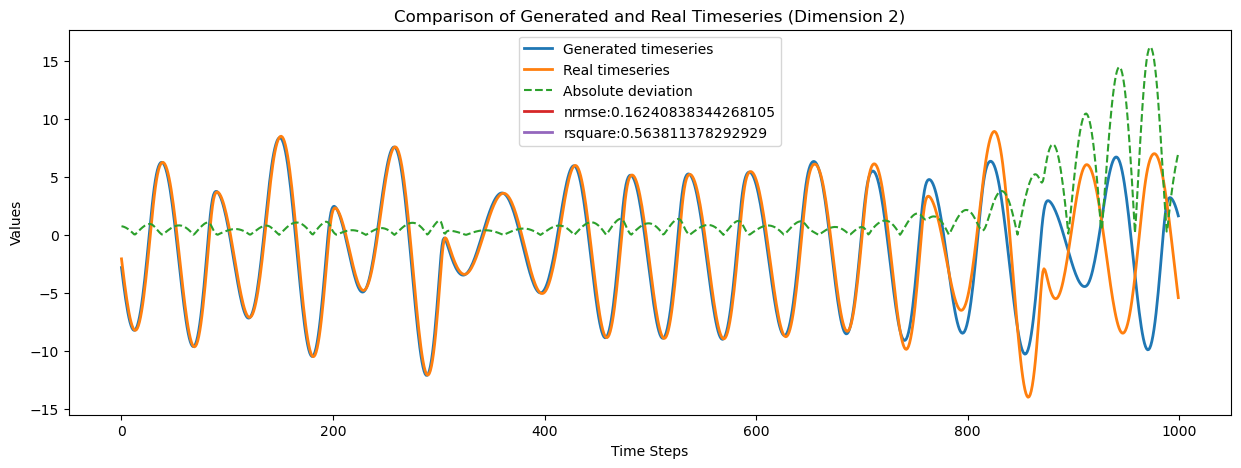
\includegraphics[width=0.7\linewidth]{Fig/10.y.png}
        \end{minipage}
        
        \vspace{.5em}
        % 画像3
        \begin{minipage}[c][.27\textheight][c]{\linewidth}
          \centering
          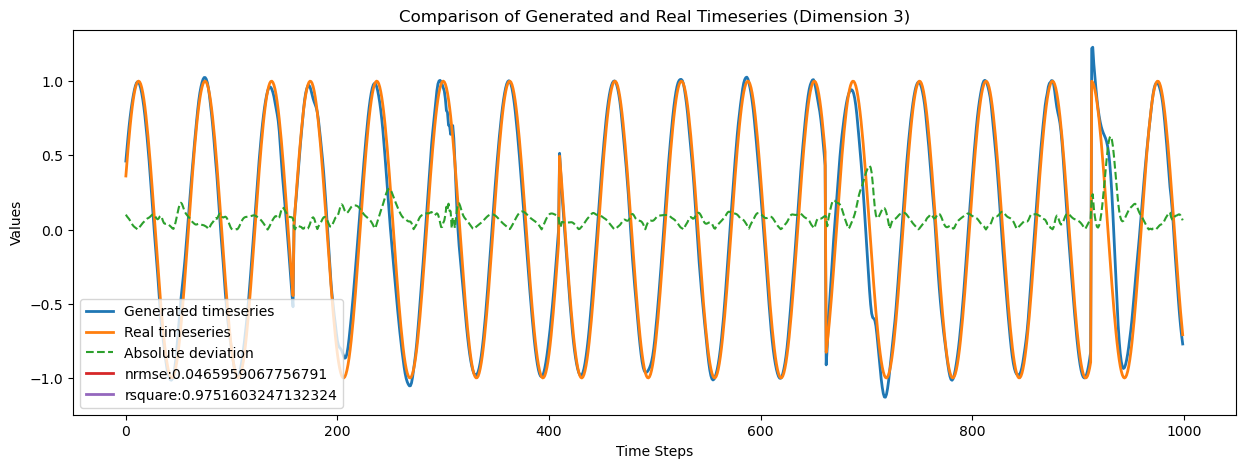
\includegraphics[width=0.7\linewidth]{Fig/10.p.png}
          \caption{\scriptsize{位相シフト(10時間分)のある外力付きRösslerモデルの予測.上から $x, y, P(t)$.}}
        \end{minipage}
      \end{figure}
    \end{column}
  \end{columns}
\end{frame}

\section{まとめと展望}
\begin{frame}
  \begin{columns}[T] % [T] は列を上部で揃えるオプション
    \begin{column}{.5\textwidth}
      \begin{figure}
        
      \end{figure}
    \end{column}
    \begin{column}{.5\textwidth}
    \end{column}
  \end{columns}
\end{frame}
